\subsection*{S4 Fig. Mesh quality assessment.}

Mesh quality was assessed using the volume-based tetrahedral distortion metric
(\texttt{tet\_qmetric\_volume}) implemented in meshtool, directly related to
the Jacobian determinant of the geometric map. The metric ranges from 0
(perfect tetrahedron) to 1 (fully degenerate element). No inverted elements
were detected in any of the 50 meshes, confirming numerical suitability for
finite element analysis.

\begin{figure}[htbp]
    \centering
    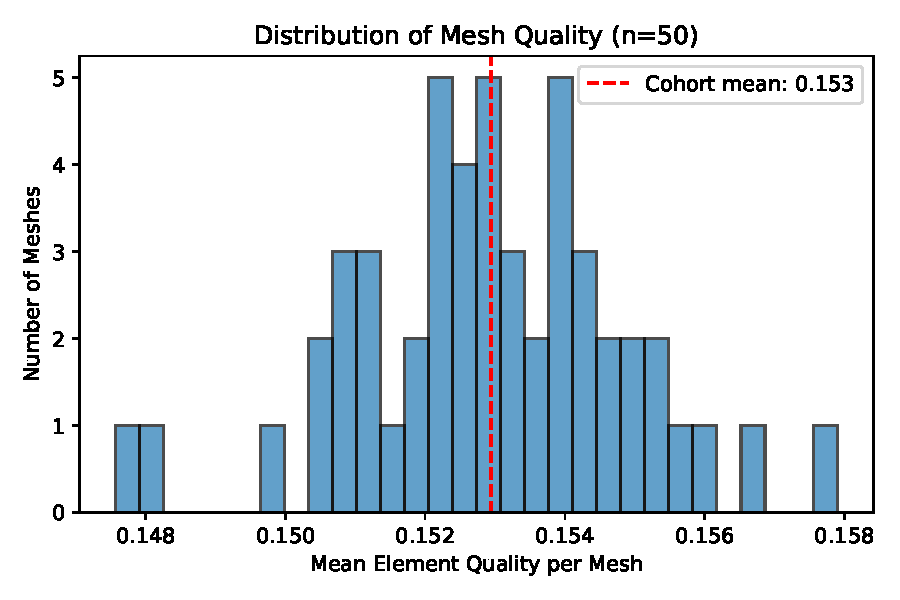
\includegraphics[width=0.8\textwidth]{pics/sp0_supp_mesh_quality_dist.pdf}
    \caption{
        \textbf{Distribution of mean element quality across the 50-heart cohort.}
        Each point represents one mesh. The \texttt{tet\_qmetric\_volume} metric
        ranges from 0 (perfect tetrahedron) to 1 (degenerate); lower values
        indicate better quality. Cohort-wide mean was $0.153 \pm 0.100$.
        No inverted elements (quality $> 0.99$) were found in any mesh.
    }
    \label{fig:s4-mesh-quality-dist}
\end{figure}

\iffalse % Table replaced by Data file (supplementary/S*_Data_mesh_quality.csv); kept here for reference only.
\begin{landscape}
\begin{longtable}{lrcccccc}
\caption{
    \textbf{Per-model mesh quality statistics for all 50 hearts.}
    Quality metric: \texttt{tet\_qmetric\_volume} (0 = perfect tetrahedron,
    1 = fully degenerate). $N_{\text{el}}$: total element count
    ($\times 10^6$). Min/Max/Mean/SD: element quality statistics per mesh.
    $N_{\text{inv}}$: inverted elements (quality $> 0.99$).
    $N_{\text{deg}}$: near-degenerate elements (quality $> 0.90$).
} \\
\toprule
\textbf{Mesh ID} &
    $N_{\text{el}}$ ($\times 10^6$) &
    \textbf{Min} &
    \textbf{Max} &
    \textbf{Mean} &
    \textbf{SD} &
    $N_{\text{inv}}$ &
    $N_{\text{deg}}$ \\
\midrule
\endfirsthead
\multicolumn{8}{c}{\tablename\ \thetable{} (continued)} \\
\toprule
\textbf{Mesh ID} &
    $N_{\text{el}}$ ($\times 10^6$) &
    \textbf{Min} &
    \textbf{Max} &
    \textbf{Mean} &
    \textbf{SD} &
    $N_{\text{inv}}$ &
    $N_{\text{deg}}$ \\
\midrule
\endhead
\midrule
\multicolumn{8}{r}{\textit{Continued on next page}} \\
\endfoot
\bottomrule
\endlastfoot
3L9ZV4XS & 2.33 & $1.56\times10^{-4}$ & 0.926 & 0.157 & 0.102 & 0 & 2 \\
591DW86I  & 2.30 & $6.15\times10^{-5}$ & 0.845 & 0.153 & 0.100 & 0 & 0 \\
5IM7QJF4  & 2.26 & $1.25\times10^{-4}$ & 0.937 & 0.152 & 0.100 & 0 & 1 \\
627ZFI97  & 2.10 & $2.15\times10^{-4}$ & 0.874 & 0.156 & 0.101 & 0 & 0 \\
66AL590N  & 2.55 & $2.22\times10^{-4}$ & 0.901 & 0.152 & 0.100 & 0 & 1 \\
6G8DD8S5  & 2.82 & $2.64\times10^{-4}$ & 0.854 & 0.151 & 0.100 & 0 & 0 \\
7D98EVAR  & 2.41 & $1.94\times10^{-4}$ & 0.895 & 0.152 & 0.100 & 0 & 0 \\
98EK6960  & 2.29 & $1.13\times10^{-4}$ & 0.950 & 0.155 & 0.101 & 0 & 5 \\
98G5I5CE  & 3.08 & $1.02\times10^{-4}$ & 0.869 & 0.153 & 0.100 & 0 & 0 \\
9HE9S8YK  & 2.85 & $2.69\times10^{-4}$ & 0.910 & 0.154 & 0.100 & 0 & 2 \\
A1VMI1BL  & 2.52 & $3.21\times10^{-4}$ & 0.891 & 0.154 & 0.101 & 0 & 0 \\
A8NCPLRI  & 4.50 & $1.18\times10^{-4}$ & 0.890 & 0.153 & 0.100 & 0 & 0 \\
B782Q8ID  & 3.20 & $3.96\times10^{-5}$ & 0.978 & 0.151 & 0.099 & 0 & 4 \\
BJRXL8KY  & 2.74 & $1.94\times10^{-4}$ & 0.955 & 0.158 & 0.102 & 0 & 6 \\
BRUN0G9V  & 2.14 & $3.88\times10^{-4}$ & 0.972 & 0.155 & 0.101 & 0 & 3 \\
C21IDK9N  & 2.51 & $9.14\times10^{-5}$ & 0.918 & 0.153 & 0.100 & 0 & 1 \\
CTW6MAJL  & 1.88 & $2.86\times10^{-4}$ & 0.875 & 0.154 & 0.100 & 0 & 0 \\
D16RF7C3  & 1.98 & $2.44\times10^{-4}$ & 0.884 & 0.154 & 0.101 & 0 & 0 \\
DA8Q81SZ  & 2.95 & $1.92\times10^{-4}$ & 0.939 & 0.151 & 0.100 & 0 & 8 \\
DHIPF4L7  & 2.21 & $3.00\times10^{-4}$ & 0.905 & 0.154 & 0.100 & 0 & 1 \\
DN98C3EZ  & 2.09 & $2.57\times10^{-4}$ & 0.949 & 0.153 & 0.100 & 0 & 1 \\
FC14      & 3.12 & $7.25\times10^{-5}$ & 0.955 & 0.151 & 0.099 & 0 & 3 \\
FC15      & 2.23 & $1.83\times10^{-4}$ & 0.956 & 0.152 & 0.100 & 0 & 4 \\
FC5       & 1.99 & $3.12\times10^{-4}$ & 0.924 & 0.152 & 0.100 & 0 & 1 \\
FC7       & 2.14 & $9.35\times10^{-5}$ & 0.918 & 0.154 & 0.100 & 0 & 2 \\
FFI8S7CY  & 2.38 & $1.76\times10^{-4}$ & 0.845 & 0.151 & 0.100 & 0 & 0 \\
FM7ID9EE  & 2.46 & $4.11\times10^{-4}$ & 0.945 & 0.153 & 0.100 & 0 & 2 \\
FQB3LGOY  & 2.38 & $1.40\times10^{-4}$ & 0.935 & 0.153 & 0.100 & 0 & 2 \\
H2JQVUUF  & 1.90 & $4.51\times10^{-4}$ & 0.912 & 0.156 & 0.101 & 0 & 1 \\
LENYCA0B  & 3.30 & $1.40\times10^{-4}$ & 0.936 & 0.151 & 0.100 & 0 & 9 \\
LLWYK03H  & 2.04 & $1.88\times10^{-4}$ & 0.939 & 0.155 & 0.101 & 0 & 5 \\
MHFn31    & 2.97 & $3.79\times10^{-4}$ & 0.854 & 0.154 & 0.101 & 0 & 0 \\
MHFw14    & 3.33 & $2.32\times10^{-4}$ & 0.915 & 0.151 & 0.099 & 0 & 1 \\
MHFw16    & 2.67 & $4.34\times10^{-4}$ & 0.869 & 0.154 & 0.100 & 0 & 0 \\
MHFw6     & 3.49 & $4.72\times10^{-5}$ & 0.835 & 0.148 & 0.098 & 0 & 0 \\
MHFw8     & 3.18 & $1.67\times10^{-4}$ & 0.891 & 0.154 & 0.101 & 0 & 0 \\
MQWINMXL  & 3.43 & $2.31\times10^{-4}$ & 0.856 & 0.148 & 0.099 & 0 & 0 \\
N4TRHUUP  & 3.66 & $9.90\times10^{-5}$ & 0.964 & 0.151 & 0.100 & 0 & 5 \\
OA15VRI2  & 2.25 & $2.33\times10^{-4}$ & 0.850 & 0.153 & 0.100 & 0 & 0 \\
OHV835G6  & 2.01 & $2.26\times10^{-4}$ & 0.878 & 0.152 & 0.100 & 0 & 0 \\
PGXLUL41  & 3.41 & $2.38\times10^{-4}$ & 0.910 & 0.154 & 0.101 & 0 & 1 \\
PJR4AHZO  & 2.38 & $3.72\times10^{-4}$ & 0.925 & 0.151 & 0.099 & 0 & 1 \\
QSBZPFZI  & 2.11 & $1.65\times10^{-4}$ & 0.876 & 0.155 & 0.101 & 0 & 0 \\
SKSXRBWF  & 2.07 & $3.59\times10^{-4}$ & 0.912 & 0.155 & 0.101 & 0 & 1 \\
TCNI6BDU  & 2.48 & $1.76\times10^{-4}$ & 0.895 & 0.153 & 0.100 & 0 & 0 \\
TNJAF3TK  & 3.01 & $2.40\times10^{-4}$ & 0.895 & 0.152 & 0.100 & 0 & 0 \\
XBTL2UYF  & 2.77 & $2.45\times10^{-4}$ & 0.869 & 0.152 & 0.100 & 0 & 0 \\
XWSQF3JX  & 2.61 & $1.49\times10^{-4}$ & 0.882 & 0.155 & 0.101 & 0 & 0 \\
Y5HYEDL4  & 2.64 & $6.21\times10^{-5}$ & 0.908 & 0.153 & 0.100 & 0 & 1 \\
YCBD3S9F  & 4.33 & $5.34\times10^{-5}$ & 0.884 & 0.150 & 0.099 & 0 & 0 \\
Z8FT2XBQ  & 2.89 & $2.06\times10^{-4}$ & 0.871 & 0.153 & 0.100 & 0 & 0 \\
\end{longtable}
\end{landscape}
\fi
